\documentclass[twoside,11pt]{article}
\usepackage{amsmath,amsfonts,amsthm,fullpage}
\usepackage{mymath}
\usepackage{algorithm}
\usepackage{algorithmic}
\usepackage{graphicx}
\usepackage{float}
\usepackage{hyperref}

\graphicspath{ {../data/} }
\newcommand{\nbs}{\texttt{nbs}}

\begin{document}

\title{CS6491-2015 P2: Swirl}
\author{Dingtian Zhang, Clement Julliard}
\date{Sep 18, 2015}
\maketitle
\begin{figure} [H]
    \centering
    
\includegraphics[width=1.0in]{pic_alan}
\end{figure}


%\begin{itemize}
%  \item Submit your answers as an electronic copy on T-square.
%  \item No unapproved extension of deadline is allowed. Zero credit will be assigned for late submissions. Email request for late submission may not be replied.
%  \item For typed answers with LaTeX (recommended) or word processors, extra credits will be given. If you handwrite, try to be clear as much as possible. No credit may be given to unreadable handwriting.
%  \item Explicitly mention your collaborators if any.
%  \item Recommended reading: PRML\footnote{Christopher M. Bishop, Pattern Recognition and Machine
%Learning, 2006, Springer.} Section 9.1, 12.1
%\end{itemize}


%----------------------------------------------------------------------------------
\section{Objective}

We want to compute the mathematical formulation and the implementation of Steady Interpolating Similarity $SIS(F_a,t,F_b)$. and validate our solution by starting with user controlled frames $F_0$ and $F_1$, by extrapolating a steady pattern of frames $F_i$ such that the transformation $T$ between $F_i$ and $F_{i+1}$ is independent of $i$, and by showing (visually) that $F_i = SIS(F_0,i/k,F_k)$ for all $i$.


\section{Definitions of Entities}


A 3D frame $\{I,J,K,O\}$ is a similarity frame if all its factors have the same magnitude, if each is orthogonal to the other two, and if $(I \times J)Ÿ \cdot K>0$.\\
\\
A Similarity Motion is an similarity frame $F(t)$ parameterize by time.\\
\\
The Steady Interpolating Similarity $SIS(F_a,t,F_b)$ is a Similarity Motion, such that:
\begin{itemize}
\item SIS(Fa,0,Fb)= Fa,
\item SIS(Fa,1,Fb)= Fb,
\item And the similarity transformation from SIS(Fa,t,Fb) to SIS(Fa,t+u,Fb) is independent of t,
\end{itemize}

\begin{figure}[h]
  \centering
  (a)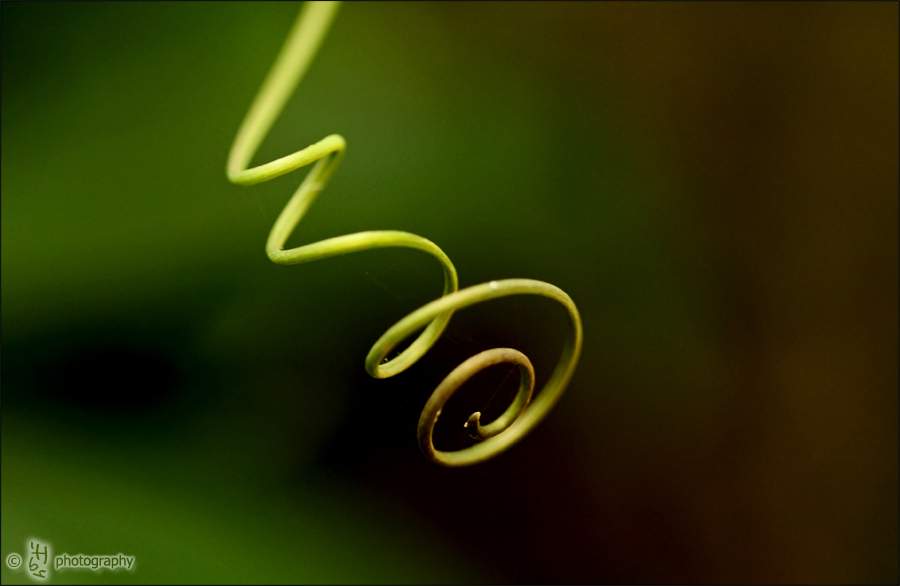
\includegraphics[width=0.46\textwidth]{plant}
  \caption{(a) Swirl in nature}
  \label{fig:time}
\end{figure}

Figure 1 shows some of the 3D swirls in nature and man-made structures.

\section{Approach}
Steady interpolating similarity motion is a combination of rotation around a fixed axis, translation along that axis, and scaling. There are many kinds of SIS motions, where rotation, translation, and scaling are different combinations. For example we have,

\subsection{Screw Motion}
Screw motion is the combination of rotation and translation. Assume the rotation is around axis $(F, N)$, initial point $P_0$, unit time rotation angle $\alpha$, speed along the axis is constant $d$, we can describe the screw motion as:
\begin{equation}
P(t) = F + FP_0^o(t\alpha) + dtN
\end{equation}
\#FIND ART\#

\subsection{Spiral Motion}
Spiral motion is the combination of rotation and scaling. One common spiral motion is log spiral. Assume the the rotation is around axis $(F, N)$, initial point $P_0$, unit time rotation angle $\alpha$, scaling factor is exponential of $m$, we can describe the log spiral motion as:
\begin{equation}
P(t) = F + m^t FP_0^o(t\alpha)
\end{equation}
\#FIND ART\#

\subsection{Swirl Motion}
Swirl motion is the combination (``commutatie composition'') of log spiral motion around an axis and exponential translation along the axis. Assume the the rotation is around axis $(F, N)$, initial point $P_0$, unit time rotation angle $\alpha$, scaling factor is exponential of $m$, velocity along the axis is exponential of $d$, we can describe the log spiral motion as:
\begin{equation}
P(t) = F + m^t FP_0^o(t\alpha, N) + d^t N
\end{equation}
\#FIND ART\#

\section{Implementation}


\subsection{Computing $N$}

For computing the $N$ from $F_0$ and $F_1$, suppose we are given the input of triangle $ABC$ and $DEF$, where $I_0 = AB, K_0 = AB \times AC, J_0 = K_0 \times I_0, I_1 = DE, K_1 =  DE \times DF, J_1 = K_1 \times I_1$, we can derive $N$ as
\begin{equation}
N = \frac{\Delta I \times \Delta J + \Delta J \times \Delta K + \Delta K \times \Delta I}{3}
\end{equation}
where $\Delta I = I_1 - I_0$, $\Delta J = J_1 - J_0$, $\Delta K = K_1 - K_0$.

\subsection{Computing $F$}
For computing the $F$ from $F_0$ and $F_1$, suppose we are given the input the same as above, we get
\begin{equation}
A = F + FA
\end{equation}
\begin{equation}
D = F + FA^o (t\alpha, N) m^t + d^t N
\end{equation}
Therefore we can derive $F$ by
\begin{equation}
A^o (t\alpha, N) m^t + d^t N - D = F^o (t\alpha, N) m^t - F
\end{equation}
where
\begin{equation}
d^t = FD \cdot N - FA \cdot N 
\end{equation}
\begin{equation}
m^t = \frac{FD - (FD \cdot N) N }{FA - (FA \cdot N) N}
\end{equation}
And rotating an arbitary point around an axis can be done by (\cite{murray13}): 

(1) Translate space so that the rotation axis passes through the origin.

(2) Rotate space about the z axis so that the rotation axis lies in the xz plane.

(3) Rotate space about the y axis so that the rotation axis lies along the z axis.

(4) Perform the desired rotation by θ about the z axis.

(5) Apply the inverse of step (3).

(6) Apply the inverse of step (2).

(7) Apply the inverse of step (1).

\subsection{Computing $F_i$ from $F_0$ and $F_1$ in 3D}
If we know $F$, $F_0$, and $F_1$, we know the swirl motion description $P(t) = F + m^t FP_0^o(t\alpha, N) + d^t N$, so we can interpolate each frame simply by changing $t$ to $2t$, $3t$, $\ldots$, $kt$.

\section{Analysis}


\section{Discussion}




\bibliographystyle{plain}
\bibliography{temp,externalPapers,groupPapers}
\begin{thebibliography}{9}
\bibitem{murray13}
  Glenn Murray,
  \emph{Rotation About an Arbitrary Axis in 3 Dimensions},
  \url{http://inside.mines.edu/fs_home/gmurray/ArbitraryAxisRotation/}.

\end{thebibliography}
\end{document}
